% Evaluation
% Related with the requirements:
% Test 1: R1: pH Control: change constant's value and verify control work

\subsection{The Circuit Setup}

\begin{figure}[h]
    \centering
    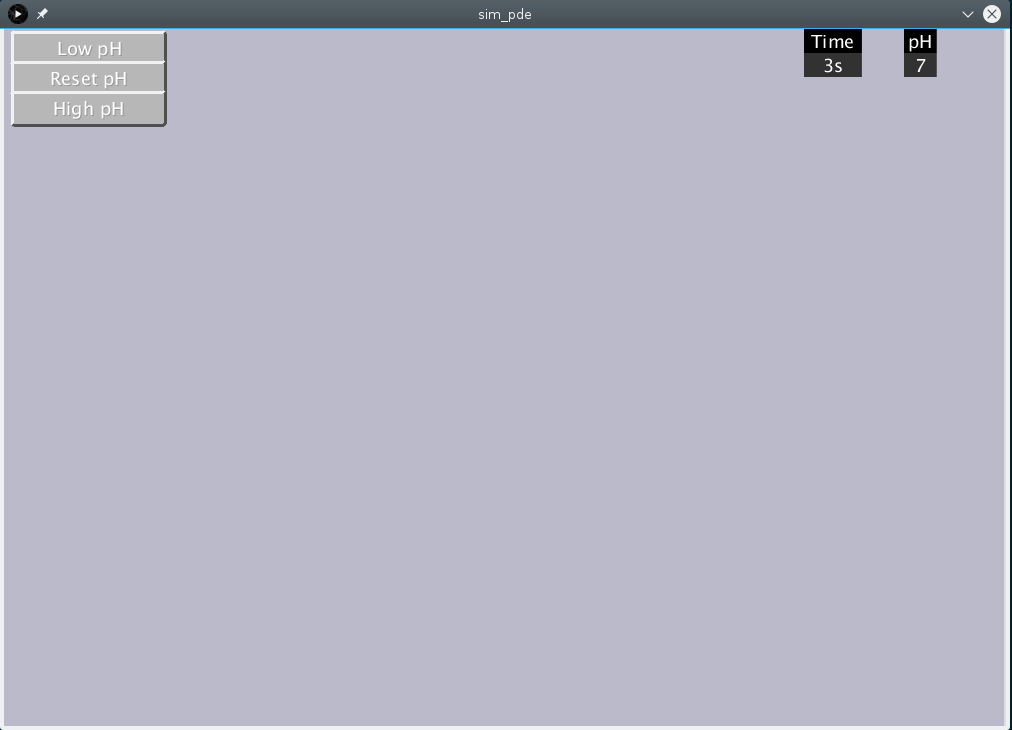
\includegraphics[width=.7\textwidth]{img/gui1.png}
    \caption{A photo of pH Control}
    \label{fig:photo}
\end{figure}

\subsection{A Graphical User Interface}

For the sake of making the unit tests to be shown in a written report,
a simple Graphical User Interface (GUI) has been implemented using Processing.
Processing is a simple programing language which is integrated with OpenGL,
Java and Serial communication.
So it is a reliable choice to display and transmit Serial data from/to Arduino within the computer screen.
But,
instead of being a monitoring-only GUI,
the Processing provides built-in functions to make mouse interactions easily,
hence the tests could be made faster.

\begin{figure}[h]
    \centering
    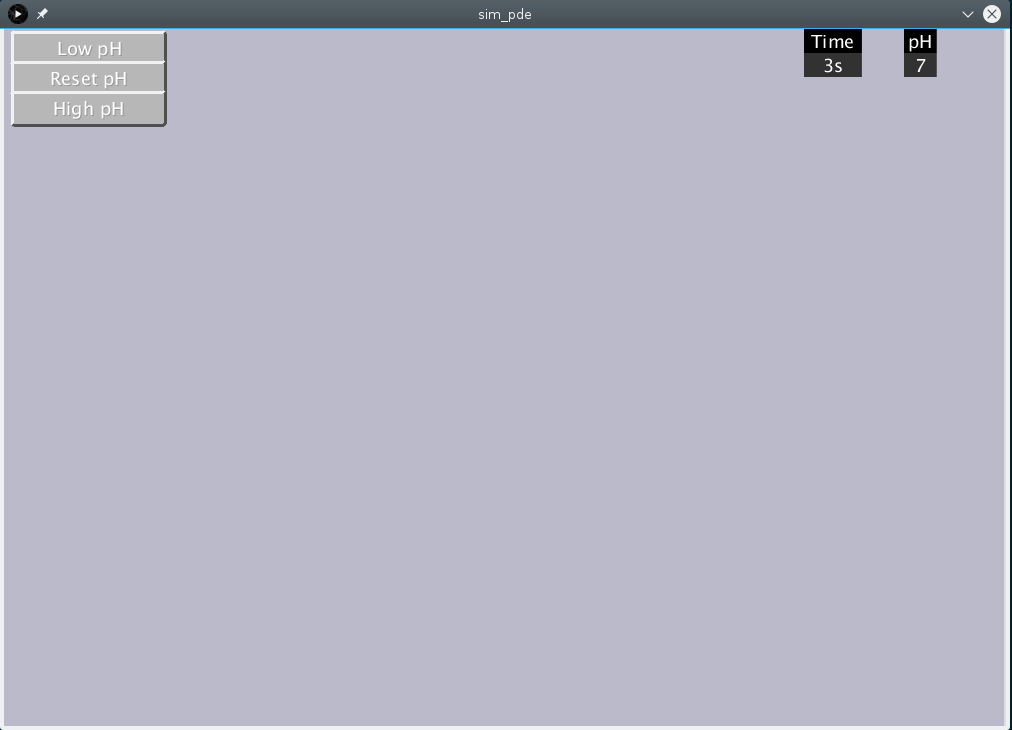
\includegraphics[width=.7\textwidth]{img/gui1.png}
    \caption{An initial version of the GUI}
    \label{fig:gui}
\end{figure}
